% Dual-Stream Architecture Figure
% Compile with: pdflatex fig_dual_stream_architecture.tex
\documentclass[tikz,border=2pt]{standalone}
\usepackage{tikz}
\usetikzlibrary{shapes.geometric, arrows.meta, positioning, fit, backgrounds, calc, decorations.pathreplacing, matrix}
\usepackage{xcolor}
\usepackage{amsmath}

% Colors
\definecolor{semanticcolor}{RGB}{65,105,225}
\definecolor{structuralcolor}{RGB}{50,150,80}
\definecolor{fusioncolor}{RGB}{150,50,150}
\definecolor{inputcolor}{RGB}{255,230,200}
\definecolor{outputcolor}{RGB}{200,255,200}

\begin{document}
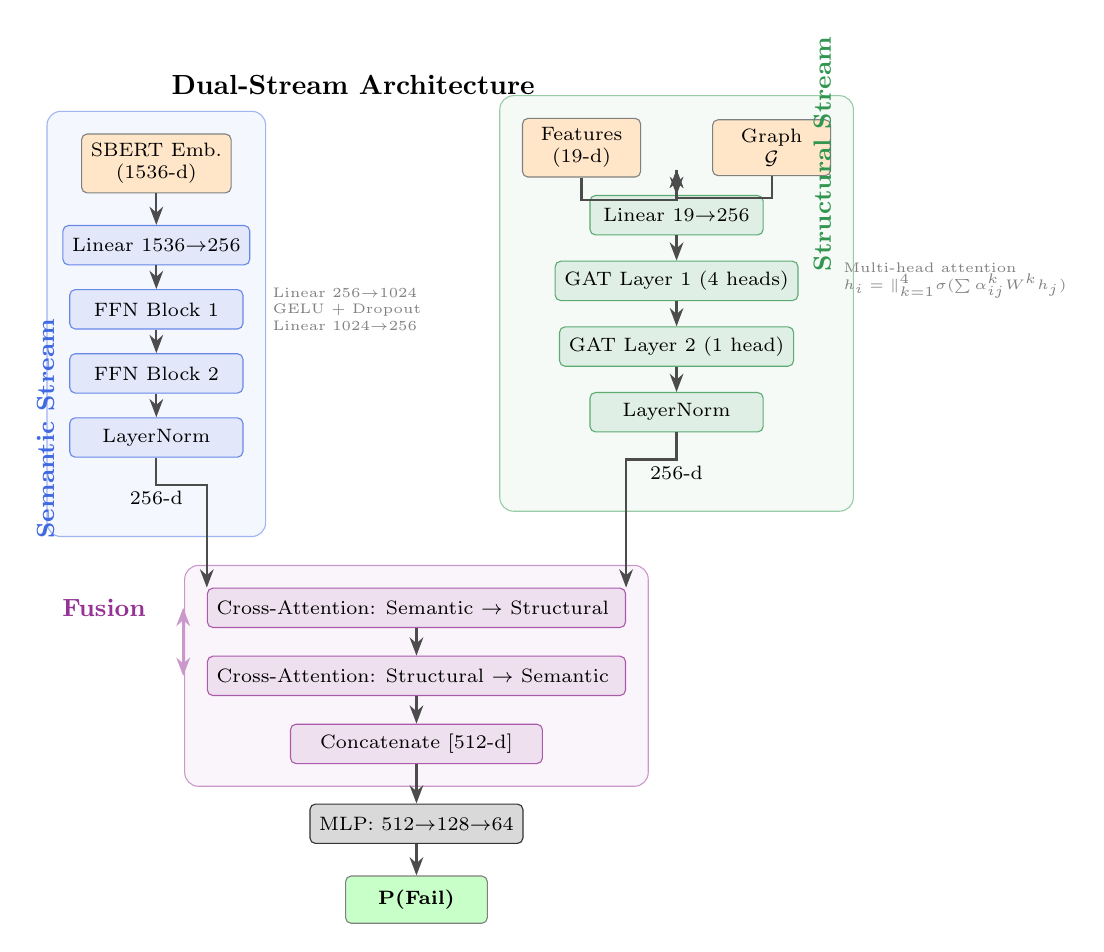
\begin{tikzpicture}[
    node distance=0.4cm,
    >=Stealth,
    every node/.style={font=\footnotesize},
    inputbox/.style={rectangle, draw=black!50, fill=inputcolor,
        minimum width=1.5cm, minimum height=0.6cm, rounded corners=2pt,
        align=center, font=\scriptsize},
    layerbox/.style={rectangle, draw=#1!80, fill=#1!15,
        minimum width=2.2cm, minimum height=0.5cm, rounded corners=2pt,
        align=center, font=\scriptsize},
    outputbox/.style={rectangle, draw=black!50, fill=outputcolor,
        minimum width=1.8cm, minimum height=0.6cm, rounded corners=2pt,
        align=center, font=\scriptsize\bfseries},
    arrow/.style={->, thick, black!70},
    streamlabel/.style={font=\small\bfseries, rotate=90},
]

% === SEMANTIC STREAM (Left) ===
\node[inputbox] (sem_in) at (0, 0) {SBERT Emb.\\(1536-d)};

\node[layerbox=semanticcolor, below=0.4cm of sem_in] (sem_proj) {Linear 1536$\rightarrow$256};
\node[layerbox=semanticcolor, below=0.3cm of sem_proj] (sem_ffn1) {FFN Block 1};
\node[layerbox=semanticcolor, below=0.3cm of sem_ffn1] (sem_ffn2) {FFN Block 2};
\node[layerbox=semanticcolor, below=0.3cm of sem_ffn2] (sem_ln) {LayerNorm};

% FFN Block detail
\node[font=\tiny, right=0.25cm of sem_ffn1, align=left, text=gray] {
    Linear 256$\rightarrow$1024\\
    GELU + Dropout\\
    Linear 1024$\rightarrow$256
};

\node[below=0.3cm of sem_ln, font=\scriptsize] (sem_out) {256-d};

% Stream label
\node[streamlabel, left=0.3cm of sem_ffn1, semanticcolor] {Semantic Stream};

\node[inputbox] (str_in) at (5.4, 0.2) {Features\\(19-d)};
\node[inputbox, right=0.9cm of str_in] (graph_in) {Graph\\$\mathcal{G}$};

\node[layerbox=structuralcolor, below=0.6cm of $(str_in)!0.5!(graph_in)$] (str_proj) {Linear 19$\rightarrow$256};
\node[layerbox=structuralcolor, below=0.32cm of str_proj] (gat1) {GAT Layer 1 (4 heads)};
\node[layerbox=structuralcolor, below=0.32cm of gat1] (gat2) {GAT Layer 2 (1 head)};
\node[layerbox=structuralcolor, below=0.32cm of gat2] (str_ln) {LayerNorm};

% Merge inputs for cleaner arrows
\coordinate (strmerge) at ($(str_proj.north)+(0,0.32)$);
\draw[arrow] (str_in.south) -- ++(0,-0.28) -| (strmerge);
\draw[arrow] (graph_in.south) -- ++(0,-0.28) -| (strmerge);
\draw[arrow] (strmerge) -- (str_proj.north);

% GAT detail
\node[font=\tiny, right=0.45cm of gat1, align=left, text=gray] {
    Multi-head attention\\
    $h_i = \|_{k=1}^4 \sigma(\sum \alpha_{ij}^k W^k h_j)$
};

\node[below=0.3cm of str_ln, font=\scriptsize] (str_out) {256-d};

% Stream label
\node[streamlabel, right=0.3cm of gat1, structuralcolor] {Structural Stream};

% === CROSS-ATTENTION FUSION ===
\node[layerbox=fusioncolor, below=1.3cm of $(sem_out)!0.5!(str_out)$, minimum width=4.2cm] (cross1) {
    Cross-Attention: Semantic $\rightarrow$ Structural
};
\node[layerbox=fusioncolor, below=0.35cm of cross1, minimum width=4.2cm] (cross2) {
    Cross-Attention: Structural $\rightarrow$ Semantic
};
\node[layerbox=fusioncolor, below=0.35cm of cross2, minimum width=3.2cm] (concat) {Concatenate [512-d]};

% Fusion label
\node[font=\small\bfseries, fusioncolor, left=0.65cm of cross1] {Fusion};

% === CLASSIFIER ===
\node[layerbox=black, below=0.5cm of concat, minimum width=2.5cm] (mlp1) {MLP: 512$\rightarrow$128$\rightarrow$64};
\node[outputbox, below=0.4cm of mlp1] (output) {P(Fail)};

% === ARROWS ===
% Semantic stream
\draw[arrow] (sem_in) -- (sem_proj);
\draw[arrow] (sem_proj) -- (sem_ffn1);
\draw[arrow] (sem_ffn1) -- (sem_ffn2);
\draw[arrow] (sem_ffn2) -- (sem_ln);

% Structural stream
\draw[arrow] (str_proj) -- (gat1);
\draw[arrow] (gat1) -- (gat2);
\draw[arrow] (gat2) -- (str_ln);

% To fusion
\draw[arrow] (sem_ln) -- ++(0,-0.6) -| (cross1.north west);
\draw[arrow] (str_ln) -- ++(0,-0.6) -| (cross1.north east);

% Cross-attention bidirectional
\draw[<->, thick, fusioncolor!50] ($(cross1.west)+(-0.3,0)$) -- ($(cross2.west)+(-0.3,0)$);

% Fusion to output
\draw[arrow] (cross1) -- (cross2);
\draw[arrow] (cross2) -- (concat);
\draw[arrow] (concat) -- (mlp1);
\draw[arrow] (mlp1) -- (output);

% === BACKGROUND BOXES ===
\begin{scope}[on background layer]
    \node[draw=semanticcolor!50, fill=semanticcolor!5, rounded corners=5pt,
          fit=(sem_in)(sem_ln)(sem_out), inner sep=8pt] {};
    \node[draw=structuralcolor!50, fill=structuralcolor!5, rounded corners=5pt,
          fit=(str_in)(graph_in)(str_ln)(str_out), inner sep=8pt] {};
    \node[draw=fusioncolor!50, fill=fusioncolor!5, rounded corners=5pt,
          fit=(cross1)(concat), inner sep=8pt] {};
\end{scope}

% === TITLE ===
\node[font=\bfseries] at (2.5, 1) {Dual-Stream Architecture};

\end{tikzpicture}
\end{document}
